% @Author: oesteban
% @Date:   2014-04-22 08:55:40
% @Last Modified by:   oesteban
% @Last Modified time: 2014-04-23 16:15:17

\documentclass[final,hyperref={pdfpagelabels=false}]{beamer}
\setbeamertemplate{bibliography item}[text]
\let\Tiny=\tiny
\providecommand\thispdfpagelabel[1]{}
\mode<presentation>{\usetheme{Blue}}

\usepackage{float}
\usepackage{glossaries}
\usepackage[english]{babel}

\usepackage[T1]{fontenc}
\usepackage{textcomp}

\usepackage[natbib=true, style=numeric-comp,backend=biber]{biblatex}

\usepackage{amsmath,amsthm, amssymb, latexsym}
\usepackage{lmodern}
\usefonttheme[onlymath]{serif}
%\boldmath
\usepackage[labelformat=empty]{caption}
\usepackage[orientation=portrait,size=a0,scale=1.4]{beamerposter}

\usepackage{graphicx,epstopdf}
\DeclareGraphicsExtensions{.pdf,.eps}
\graphicspath{{../figures/} {logos/}}

\usepackage{array,booktabs,tabularx}
\newcolumntype{Z}{>{\center\arraybackslash}X}
%\newcolumntype{Z}{>{\centering\arraybackslash}X} % centered tabularx columns
%\newcommand{\sups}[1]{\ensuremath{^{\textrm{#1}}}}
%\newcommand{\subs}[1]{\ensuremath{_{\textrm{#1}}}}
%\newcommand{\pphantom}{\textcolor{ta2skyblue}} % phantom introduces a vertical space in p formatted table columns??!!
\usepackage[scaled=.7]{beramono}


\bibliography{99-references}
\appto\bibfont{\hskip1cm\tiny}

\DeclareSymbolFont{cmlargesymbols}{OMX}{cmex}{m}{n}
\let\sumop\relax
\DeclareMathSymbol{\sumop}{\mathop}{cmlargesymbols}{"50}

\listfiles

%%%%%%%%%%%%%%%%%%%%%%%%%%%%%%%%%%%%%%%%%%%%%%%%%%%%%%%%%%%%%%%%%%%%%%%%%%%%%%%%%%%%%%

 
\title{\huge Simulation-based evaluation of susceptibility distortion correction methods in dMRI}
\author[Esteban et al.]{O. Esteban$^{1,2}$\and%
A. Daducci$^{2}$\and%
E. Caruyer$^{3}$\and%
K. O'Brien$^{4}$\and%
MJ. Ledesma-Carbayo$^{1}$\and%
M. Bach-Cuadra$^{5,2}$\and%
A. Santos$^{1}$}%}
\institute{
$^{1}$~
\includegraphics[height=2cm]{logos/BIT.pdf}~
\includegraphics[height=2cm]{logos/UPM.pdf}\hfill%
$^{2}$~
\includegraphics[height=2cm]{logos/LTS5.pdf}~
\includegraphics[height=2cm]{logos/EPFL.pdf}\hfill%
$^{3}$~
\includegraphics[height=2cm]{logos/SBIA.pdf}~
\includegraphics[height=2cm]{logos/Penn.pdf}\hfill%
$^{4}$~
\includegraphics[height=2cm]{logos/CIBM.pdf}~
\includegraphics[height=2cm]{logos/UNIGE.pdf}\hfill%
$^{5}$~
\includegraphics[height=2cm]{logos/CHUV.pdf}~
\includegraphics[height=2cm]{logos/UNIL.pdf}%
}
\date[May 5th, 2012]{May 5th, 2012}

%%%%%%%%%%%%%%%%%%%%%%%%%%%%%%%%%%%%%%%%%%%%%%%%%%%%%%%%%%%%%%%%%%%%%%%%%%%%%%%%%%%%%%
\newlength{\columnheight}
\setlength{\columnheight}{102cm}

% List of acronyms used in the text
\newacronym{mr}{MR}{magnetic resonance}
\newacronym{mri}{MRI}{magnetic resonance imaging}
\newacronym{dmri}{dMRI}{diffusion MRI}
\newacronym{fmri}{fMRI}{functional MRI}
\newacronym{dw}{DW}{diffusion weighted}
\newacronym{dti}{DTI}{diffusion tensor imaging}
\newacronym{t1}{T1}{T1-weighted}
\newacronym{t2}{T2}{T2-weighted}
\newacronym{csf}{CSF}{cerebrospinal fluid}
\newacronym{wm}{WM}{white matter}
\newacronym{gm}{GM}{grey matter}
\newacronym{epi}{EPI}{echo-planar imaging}
\newacronym{gre}{GRE}{gradient echo sequence}
\newacronym{fa}{FA}{fractional anisotropy}
\newacronym{md}{MD}{mean diffusivity}
\newacronym{adc}{ADC}{apparent diffusion coefficient}
\newacronym{acwe}{ACWE}{active contours without edges}
\newacronym{adf}{ADF}{active deformation field}
\newacronym{map}{MAP}{maximum a posteriori}
\newacronym{snr}{SNR}{signal-to-noise ratio}
\newacronym{pve}{PVE}{partial volume effect}
\newacronym{roi}{ROI}{region of interest}
\newacronym{mrf}{MRF}{Markov Random Field}
\newacronym{psf}{PSF}{point-spread function}
\newacronym{se}{SE}{Surface error}
\newacronym{wi}{WI}{Warping index}
\newacronym{nof}{NoF}{number of fibers}
\newacronym{hardi}{HARDI}{high angular resolution diffusion imaging}
\newacronym{tpm}{TPM}{tissue probability map}
\newacronym{fft}{FFT}{fast fourier transform}
\newacronym{vsm}{VSM}{voxel shift map}

\newacronym{fmb}{FMB}{fieldmap-based}
\newacronym{reb}{REB}{reversed encoding-based}
\newacronym{t2b}{T2B}{T2 registration-based}

\newacronym{frr}{FRR}{fiber recovery ratio}

\makeglossaries

%\acrodef{mr}[MR]{magnetic resonance}
%\acrodef{mri}[MRI]{magnetic resonance imaging}
%\acrodef{dwi}[DWI]{diffusion weighted imaging}
%\acrodef{dw}[DW]{diffusion weighted}
%\acrodef{dti}[DTI]{diffusion tensor imaging}
%\acrodef{t1}[T1]{T1-weighted}
%\acrodef{t2}[T2]{T2-weighted}
%\acrodef{csf}[CSF]{cerebrospinal fluid}
%\acrodef{wm}[WM]{white matter}
%\acrodef{gm}[GM]{grey matter}
%\acrodef{epi}[EPI]{echo-planar imaging}
%\acrodef{fa}[FA]{fractional anisotropy}
%\acrodef{md}[MD]{mean diffusivity}
%\acrodef{acwe}[ACWE]{active contours without edges}
%\acrodef{map}[MAP]{maximum a posteriori}
%\acrodef{snr}[SNR]{signal-to-noise ratio}
%\acrodef{pve}[PVE]{partial volume effect}
%\acrodef{roi}[ROI]{region of interest}


\begin{document}

\begin{frame}[t]
  \noindent\makebox[\textwidth][c]{%}
  \begin{minipage}[t][\columnheight][c]{0.95\textwidth}
  \parbox[t][\columnheight][c]{\textwidth}{%
  \begin{columns}[t,totalwidth=\textwidth]
    \begin{column}{.34\linewidth}
      \begin{beamercolorbox}[center,wd=\textwidth]{postercolumn}
        \begin{minipage}[T]{.95\textwidth}  % tweaks the width, makes a new \textwidth
          \parbox[t]{\textwidth}{ % must be some better way to set the the height, width and textwidth simultaneously
            % Since all columns are the same length, it is all nice and tidy.  You have to get the height empirically
            % ---------------------------------------------------------%
            % fill each column with content            
            \begin{alertblock}{}
              \begin{itemize}
                \item Connectivity analyses rely on complex workflows to extract the network from dMRI datasets.
                \item One important pitfall that potentially bias the extracted connectome is susceptibility
                      distortion, a typical artifact on dMRI [Irfanoglu et al. 2012].
                \item In this work, we evaluate three widely used methodologies for bias correction, originally
                      proposed for fMRI data:
                      fieldmap-based method (FMB, [Jezzard et al 1995]),
                      reverse-encoding method (REB, [Cordes et al. 2000, Chiou et al. 2000]),
                      and T2-weighted intensity-based registration (T2B, [Kybic et al. 2000]).
                \item Benchmarking includes geometrical accuracy scores, signal recovery scores, and
                      a preliminary study of impact on the extracted tractography and connectivity matrices.
              \end{itemize}
            \end{alertblock}
          }
        \end{minipage}
      \end{beamercolorbox}
    \end{column}
    % ---------------------------------------------------------%
    % end the column

    % ---------------------------------------------------------%
    % Set up a column 
    \begin{column}{.64\linewidth}
      \begin{beamercolorbox}[center,wd=\textwidth]{postercolumn}
        \begin{minipage}[T]{.95\textwidth} % tweaks the width, makes a new \textwidth
          \parbox[t]{\textwidth}{ % must be some better way to set the the height, width and textwidth simultaneously
            % Since all columns are the same length, it is all nice and tidy.  You have to get the height empirically
            % ---------------------------------------------------------%
            % fill each column with content
	        \begin{block}{Digital dMRI phantom \& theory-based warping}
          We generated a test set using low-resolution dMRI phantoms (online available$^{1}$)
          with corresponding T1-weighted and T2-weighted images at high-resolution.

          We simulate the artifact (geometrical distortion and signal dropout) using a synthetic fieldmap.
              \begin{figure}[thpb]
                 \centering
                 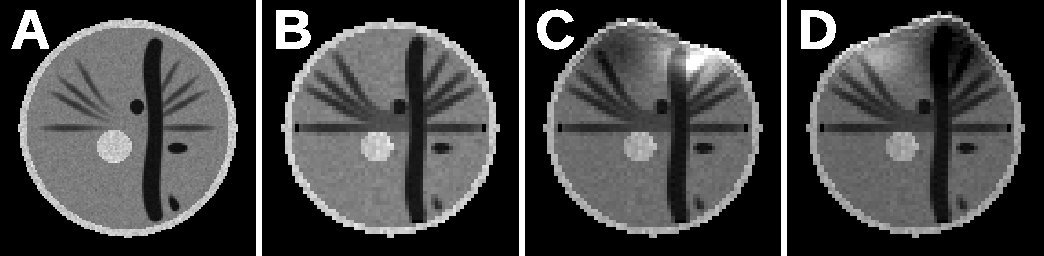
\includegraphics[width=0.95\columnwidth]{Fig01-Phantom}
              \end{figure}
              A) T2w; B) undistorted \textit{b0} volume;
                 C, D) distorted \textit{b0} volumes with opposed phase 
                 encoding directions, maximum displacement of 3.80~mm.
          \end{block}

          \begin{block}{Evaluation framework}
          We use \emph{nipype}$^{2}$, a powerful tool for building processing pipelines in
          neuroimaging.

          The evaluation framework includes the phantom distortion module, the three correction
          methodologies, DTI\&HARDI reconstruction methodologies, tractography,
          and a final module to analyse downstream impact on geometry, tractography and connectivity.
          \end{block}
          }
          % ---------------------------------------------------------%
          % end the column
        \end{minipage}
      \end{beamercolorbox}
    \end{column}
    % ---------------------------------------------------------%
    % end the column
  \end{columns}
  \vfill
  \noindent\makebox[\textwidth][l]{
  \begin{minipage}{0.978\textwidth}
      \begin{beamercolorbox}[]{postercolumn}
            \begin{block}{Visual results}
              \begin{figure}
                 \centering
                 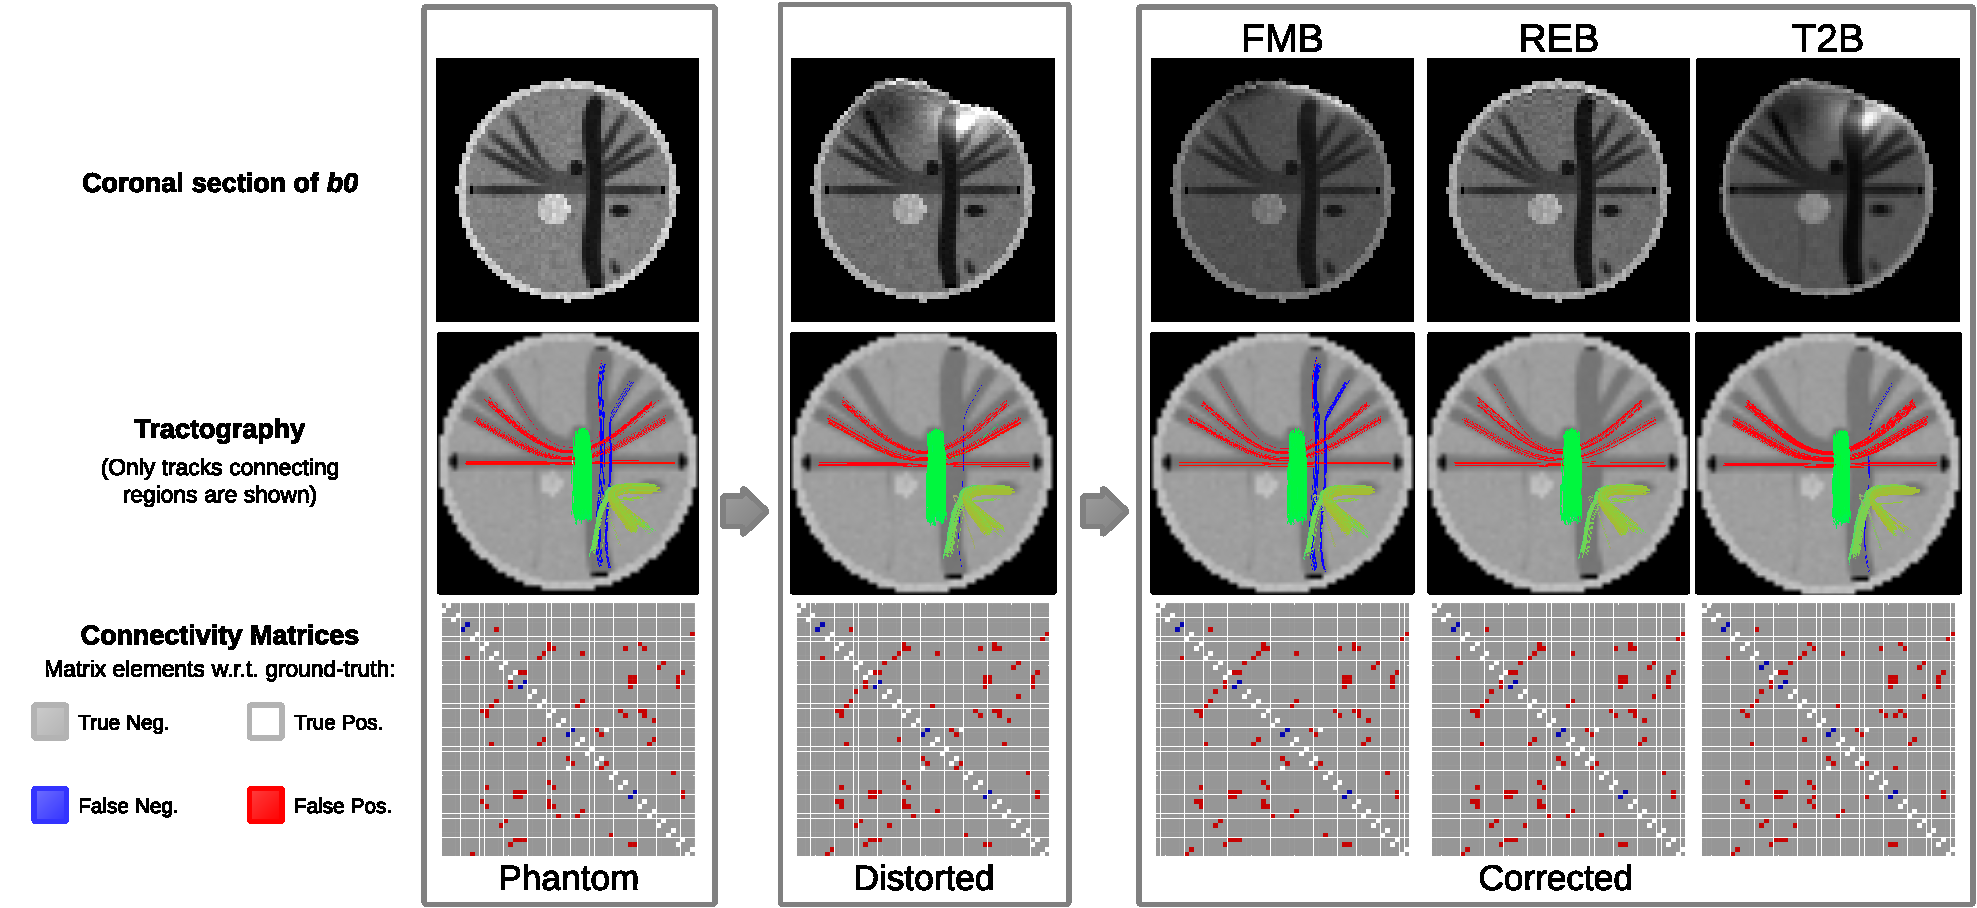
\includegraphics[width=\textwidth]{Fig02-Results}
              \end{figure}
            \end{block}
      \end{beamercolorbox}
  \end{minipage}
  }
  \vfill
  \begin{columns}[T,totalwidth=\textwidth]
    \begin{column}{.34\textwidth}
      \begin{beamercolorbox}[center,wd=\textwidth]{postercolumn}
        \begin{minipage}[T]{\textwidth}  % tweaks the width, makes a new \textwidth
          \noindent\parbox[t]{\textwidth}{ % must be some better way to set the the height, width and textwidth simultaneously
            % Since all columns are the same length, it is all nice and tidy.  You have to get the height empirically
            % ---------------------------------------------------------%
            % fill each column with content
            \vfill            
            \begin{block}{Quantitative results}
            \noindent\makebox[\textwidth][c]{%}
            \begin{minipage}[T][][c]{.75\textwidth} 
            
\begin{table}[h]
\caption{Numerical results}
\label{table:results}
\begin{center}
\begin{tabular}{c||cc|cccc}
\hline
Method & \multicolumn{2}{c|}{Similarity (\%)} & \multicolumn{4}{c}{\gls*{fji} (\%)} \\
\hline
 & B0 & \glspl*{dwi} & Av. & \gls*{csf} & \gls*{wm} & \gls*{gm} \\
\hline
\gls*{fmb} & $80.05$ & $96.26\pm.06$ & $93.00$ & $88.57$ & $96.74$ & $94.02$ \\
\hline
\gls*{reb} & $91.00$ & $97.65\pm.03$ & $96.64$ & $94.31$ & $98.26$ & $96.75$ \\
\hline
\gls*{t2b} & $64.58$ & $90.10\pm.13$ & $79.19$ & $66.31$ & $89.85$ & $82.14$ \\
\hline
\end{tabular}
\end{center}
\end{table}
            
\begin{table}[!t]
\caption{Tractography and connectivity results.}
\label{table:results-tractography}
\begin{center}
\begin{tabular}{l||cccc}
\hline
 & \# tracks & length (mm) & FP & FN \\
\hline
Original & 735 & $40.87\pm13.55$ & 40 & 4 \\
\hline
Distorted & 878 & $40.54\pm13.73$ & 42 & 4 \\
\hline
\gls*{fmb} & 743 & $40.04\pm13.60$ & 43 & 4 \\
\hline
\gls*{reb} & 830 & $39.87\pm13.93$ & 44 & 4 \\
\hline
\gls*{t2b} & 825 & $41.44\pm12.85$ & 40 & 5 \\
\hline
\end{tabular}
\end{center}
\end{table}
            \end{minipage}
            }
            \end{block}
            \vfill
            \begin{exampleblock}{}
            \begin{figure}
                \centering
                \begin{minipage}{0.45\textwidth}
                \centering
                
\includegraphics[height=3.5cm]{logos/qrcode-github}
                \caption{\tiny My GitHub}
                \end{minipage}\hfill
                \begin{minipage}{0.45\textwidth}
                \centering
                
\includegraphics[height=3.5cm]{logos/qrcode-paper}
                \caption{\tiny Paper}
                \end{minipage}
                \end{figure}
            \end{exampleblock}
          }
        \end{minipage}
      \end{beamercolorbox}
    \end{column}
    % ---------------------------------------------------------%
    % end the column

    % ---------------------------------------------------------%
    % Set up a column 
    \begin{column}{.64\textwidth}
      \begin{beamercolorbox}[center,wd=\textwidth]{postercolumn}
        \begin{minipage}[T]{.95\textwidth} % tweaks the width, makes a new \textwidth
          \parbox[t]{\textwidth}{ % must be some better way to set the the height, width and textwidth simultaneously
            % Since all columns are the same length, it is all nice and tidy.  You have to get the height empirically
            % ---------------------------------------------------------%
            % fill each column with content
          \begin{block}{Conclusions and references}
            \begin{itemize}
              \item In terms of geometry, REB ranked first.
              \item In terms of tractography, visual assessment and
                    quantitative results suggested that FMB and REB perform better.
              \item Only HARDI yielded useful results. DTI-based tractography erroneously
                    estimated crossing and kissing fibers, therefore it was discarded
                    from evaluation.
              \item Connectivity matrices from HARDI were evaluated. Still, a more appropriate
                    phantom is required, presenting its connecting interface
                    densely covered by the seeding regions.
              \item Connectome analyses demand the standardization of
                    processing techniques and pipelining sofware tools to
                    ensure the reproducibility of experiments and the 
                    reliability of results.
            \end{itemize}

            \noindent{\vskip1cm\textbf{Links and references}}\par
            \begin{enumerate}
            \item {\small\url{emmanuelcaruyer.com/phantomas.php}}\par
            \item {\small\url{nipy.sourceforge.net/nipype}}
            \end{enumerate}
          \end{block}
          }
          % ---------------------------------------------------------%
          % end the column
        \end{minipage}
      \end{beamercolorbox}
    \end{column}
    % ---------------------------------------------------------%
    % end the column
  \end{columns}
%  }
  %\vfill
  %\begin{alertblock}{}
  %    1. {\small\url{emmanuelcaruyer.com/phantomas.php}} \par
  %    2. {\small\url{nipy.sourceforge.net/nipype}}
  %\end{alertblock}
  }
  \end{minipage}
}
\end{frame}

\end{document}